% --------------------------------------------------------------
% This is all preamble stuff that you don't have to worry about.
% Head down to where it says "Start here"
% --------------------------------------------------------------
 
\documentclass[12pt]{article}
 
\usepackage[margin=1in]{geometry} 
\usepackage{amsmath,amsthm,amssymb}
\usepackage{graphicx}
\usepackage{enumitem}
\usepackage{subcaption}
\usepackage{url}

\begin{document}
 
% --------------------------------------------------------------
%                         Start here
% --------------------------------------------------------------
 
\title{PROJECT 2}%replace X with the appropriate number
\author{ECE759 Pattern Recognition-Spring 2016\\ %replace with your name
Laura Gonzalez\\Charles West\\Selene Schmittling\\} %if necessary, replace with your course title
 
\maketitle

\section{Introduction}

In this project we utilize the dataset used in Project 1.  This data set includes two groups of images: one set are labeled "Water" images and the other is labeled "Non-water" images. In project 1, the images were manually cropped and water pixels labeled for both sets of images. \\
\\
In this project we are tasked with
\begin{itemize}
	\item defining an architecture for and running a Neural Network for classification;
	\item defining appropriate parameters for and implementing a support vector machine.
	\item identifying feature vectors that can describe water vs. non-water and using techniques to determine if the feature vectors are "good".
	\item proposing an unsupervised classification technique to classify regions into two clusters.
\end{itemize}
In this section, we briefly describe the techniques we explored in general. In the Methodology section, we describe our specific implementations and in Results, we describe the results of our systems and compare them to the Bayes classifier we used in the first Project. 
\subsection{Neural Network}
Convolutional neural networks ('CNNs') deliver state of the art performance in image classification and segmentation, delivering strong results with large datasets such as ImageNet.  There are a few key factors that have allowed CNNs to reach this level of performance.  It is well known that increasing the amount of training data provided to a good method increases performance and generalization.  Neural networks are capable of productively utilizing nearly unlimited amounts of training data, primarily constrained by memory and processing speeds.\\
\\
CNNs are especially well-suited to image processing due to their spacial coherence.  Rather than using fully connected neurons which examine the whole image at once (thereby introducing a extremely large number of parameters), CNNs learn filters instead which are then applied to the full image.  This drastically reduces the number of parameters per layer of the network and introduces natural translation invariance due to the identical treatment of each pixel (since the filter is applied at every offset in the network).  This approach evolves filters that have been identified as similar to the filters that have been manually produced in computer vision literature via exhaustive analysis, while producing new and interesting filters that had not been previously identified in higher layers.  Since some of these filters/features appear to be universal among images (such as edge detection), it has become a common practice to take layers with pre-trained weights from top performing networks and then retrain with other top layers and data sets to create new classifiers.  This practice allows much smaller training sets to be used that are still able to generate good/generalizable results, essentially borrowing features from otherwise unrelated training data.\\
\\
CNNs work extremely well for complex images and scenes but require large amounts of data (unless the layer borrowing method is used), since the network is essentially having to recreate how vision works from scratch when it starts training.  It is normal for the training sets for these networks to be on the order of a million images.  There are roughly 70 training/test images for this project, which implies that CNNs (and other methods) might have difficulty generalizing.\\
\\
One of the key enabling factors for the high performance of modern neural networks is their ability to use high power GPUs to reduce training time by a factor of 100 or more.  This allows the networks to both have high complexity and handle large amounts of data.  However, this GPU dependence also makes it significantly more difficult to setup and train large neural networks because specialized/experimental libraries and expensive hardware required to get fast results.  Effectively, training CNNs requires a certain amount of software engineering expertise just to get started.\\
\\
\subsection{Support Vector Machine ("SVM")}
Support Vector Machines are another technique used to classify data. When classifying linearly separable data, SVM maximizes the distance between the two classes which improves generalizability for new data. In essence, it creates the maximum buffer between the classes so that testing points are more accurately assigned to their appropriate class. In the case of non-separable data, the algorithm adds an additional constraint of minimizing the mis-classification that occurs in the training data. Convex optimization is at the root of SVM's optimality\cite{haykin2009neural}.\\
\\
In cases where classes are non-linearly separable, we are able to employ kernels which convert the given feature space to a higher dimensional and hopefully more separable space. Popular kernel functions include polynomials, radial basis functions and the hyperbolic tangent\cite{theodoridis2009pattern}.
\subsection{Feature Selection}
Feature selection is a key process in classifying data. Some features will be better suited to a classification problem then others. Ideal features will linearly separate the classes such that data points in the same cluster are close together and data points in different clusters are far apart. Even if the features are not linearly separable, it will be best if they are able to separate the classes in space.\\
\\
One of the issues involved in trying to identify whether features are well chosen is that the vectors are frequently larger than 3 in dimension which means there is no way to visualize the data points in relation to each other. One of the measures that can be used to identify how well spaced data points are is to use scatter matrices and calculations which use them. Scatter matrices quantify the between cluster and within cluster distance. Feature vectors for which the within cluster distance is very small (low variance) and for which between cluster distance is large (i.e., the data is very separated) is desirable. \\
\\
Additional information can be gained from calculations with utilize information in these matrices. \\
\\
Another tool that can be used to deal with feature vectors is Principal Components Analysis (PCA). PCA quantifies the axis along which maximal variance in the data points occurs. It is possible to identify these axes and a basis which more separates the data. 
\subsection{Unsupervised classification}
Unsupervised classification is used in cases where labels are not available. Unsupervised methods include: sequential, hierarchical, hard clustering, fuzzy clustering, boundary detection algorithms and ones which perform cost optimization. Each of these methods requires the choice of certain parameters. The optimal values for these parameters are not always easily identifiable. An additional issue with unsupervised classification is identifying the significance of the generated clusters. It is frequently difficult to describe the meaning of the clustering in the context of the data. The significance is highly data-dependent. For instance. clusters of gene expression data has been associated with genes which are involved in the same process (co-expressed). It is unclear what the clusters mean for color spaces. However, when we clustered water pixels exclusively in Project 1, it seemed as if the clusters corresponded to "shadows".

\section{Methodology}
\subsection{Neural Networks}
\subsubsection{Convolutional Neural Networks}
To implement a CNN, we utilized a couple of different C++ libraries which we embedded in implmentation code we developed during Project 1.
\subsubsection{Neural Network Libraries}
	Two neural network libraries where considered and used for this project:\\
\begin{enumerate}
	\item TinyCNN is a header only C++ library which advertises its ease of integration/use (minimal dependencies).  It supports feed forward neural networks without skip layers and  multi-threaded CPU based training, but does not allow GPU based training.  It has minimal support for image processing, with one or two examples of how to read data from an OpenCV Mat image class \cite{tinyCNN}.  \\
	\item Caffe is a full featured library which focuses on GPU accelerated CNNs and language-independent sharing of trained networks.  It supports feed forward networks with relatively arbitrary architectures (including skip layers) and supports both single CPU training and training on one or more GPUs.  Working with the library revealed that it has a strong focus on image classification which can make it somewhat difficult to use for image segmentation due to some assumptions in the library code.  Caffe has a large number of dependencies and requires recent versions of its dependency libraries \cite{caffe}.\\
	Given the limited amount of time available for completing the project, a plan was formed to get some working results using the TinyCNN library and then explore what would be needed to train a more sophisticated network with Caffe since it seemed likely that it would take significant effort to get Caffe working.
\end{enumerate}
\subsubsection{Initial Neural Network Classifier}
	The C++ framework which had been written for project 1 was reused and a new “NeuralNetworkClassifier” class was added.  The framework allows subclasses of the base class “classifierBaseClass” to define “train” and “segment” functions and then automatically presents them with image data.  Since there was some uncertainty with the ordering of the data required to use TinyCNN's CNN layers (since they have spacial dependence), the images where instead broken up into a set 5x5 chunks (one for each pixel, with its neighbors) and presented to a fully connected neural network.\\
\\
	The initial network was trained for 24 hours on a Thinkpad laptop and then the results were analyzed.  The segmentations produced by the initial classifier were completely blank.  Tweaking the parameters and retraining didn't produce better results, so it was decided that it would be preferable to start with a system that was easier to debug and then move to the large scale system.
\subsubsection{Network Design Considerations}
	A supervised learning method is essentially a function approximator, so we implemented a fully connected neural network to approximate a sine function as an initial test task.  The shorter training time of this simple case allowed more exploration of how network architectures, activation functions, loss functions, dropout and solver strategies affected results and training time.  There were a number of different methods available in the library but few clear guides in the literature on how to choose between them.\\
\\
	Sigmoid activation functions were popular for much of the neural network research conducted previous to the advent of “deep learning”.  Recent literature appears to indicate that sigmoid activation functions have theoretical properties which tend to result in a “vanishing gradient” which makes it difficult to train deep sigmoid networks.  It has been suggested that hyperbolic tan-based activation functions should nearly always be used in applications in which sigmoid activations where previously employed due to their greater resistance to the vanishing gradient problem \cite{tanHForumPost}.\\
\\  
	Rectified linear functions are a more recently developed family of activation functions which have enjoyed considerable success in many areas.  They are essentially the max(input sum, 0), which means that their gradient is very fast to compute (because it is either 0 or 1).  They don't suffer from the vanishing gradient problem.  Their primary drawback (which also been cited as an advantage) is that nodes can “switch off” once their inputs go consistently below 0 and their gradient goes to 0 \cite{glorot2011deep}.  This results in sparse networks once training finishes. However, there are some concerns that nodes could be “switched off” too early in the training.  “Leaky Rectified Linear Units” are an alternative to rectified linear units which maintain a small but finite gradient when they would normally be “switched off”.  This prevents the development of sparse networks.  It has also been claimed that it is beneficial to add another parameter which trains the gradient of the unit (called “PRelu”), but it is not clear that it has advantages over leaky rectified linear units.\\
\\
	It has been proven that a sufficiently large two layer sigmoid or hyperbolic tangent network is capable of representing any function.  However, one of the insights of “deep learning” is that deeper networks can have better generalization for a given training set/training time (if your network does not suffer from vanishing gradient).  While this would seem to indicate that it would be best to use very deep networks,  they can take a long time to train and it would appear to be problem dependent as to what depth is best.\\
\\
	One of the more traditional loss functions is the squared difference between the expected output of the network and its actual output (mean squared error).  It has been criticized for not punishing large deviations sufficiently and tends not to be used for classification.  Instead, the cross-entropy loss function is widely recommended for classification problems (such as segmentation).\\
\\
	Dropout is a widely recommended regularization method which is known to increase the generalization of a network.  It operates by randomly dropping nodes from the network, thereby forcing the network to be resilient and punishing delicate complex interactions between nodes by forcing them to operate in a noisy environment.  Once training has been completed, the weights of the network are scaled and all of the nodes are used.  This should result in a network that approaches the consensus of a large number of different possible network architectures and should converge on the general model for the function of interest \cite{srivastava2014dropout}.\\
\\
	Neural networks can be trained by a wide variety of methods.  That said, most of the methods that are used in practice are based on a form of gradient descent because it appears to be one of the few approaches that works well for large scale networks and data.  Pure gradient descent is still (surprisingly) widely used.  It is common to improve basic gradient descent by adding a momentum term and using learning rate annealing, which helps with getting in the approximately correct global region and finding the local minimum respectively. There are also a number of solvers which operate by controlling the learning rate via other measures, often using lightweight approximations of the gradient change rate \cite{gradientDescentMethods}.  Many of these methods (such as ADAM) are available for use in modern neural network libraries.\\
\\
	Due to the initial neural network classifier failing to produce results and the dizzying number of possible architectures and parameters, a simpler problem was explored to determine a configuration that might be feasible for the larger problem.  A sine function was sampled at a step size of .001 and used as training data for the prototype network.  Since rectified linear units (RELU) have been praised in the literature for training speed and cross-entropy is praised for classification tasks, initial experiments where carried out using a 50 unit per layer (RELU, RELU, linear) network with a cross-entropy loss function.  This resulted in all zero output despite training for an hour on the complete sine data set.  Changing the solver (ADAM, gradient descent, etc) settings did not appear to help the problem.\\
\\
	RELU is known for “turning off”, so leaky RELU and PRELU where tried.  Neither appeared to work.  However, changing the loss function from cross-entropy to mean squared error allowed the network to train (a difficult that has been noted by others \cite{crossEntropyWithRELU}.  This in turn allowed the network to approximate the sine function for the first half of its domain, but was not able to approximate the remainder (even with a large training time).  Deeper networks were tried and helped somewhat but did not improve the local minimum problem.  Switching to other solvers helped considerably, eventually allowing a high quality sine approximation in under 5 seconds of training (a marked improvement over gradient descent).\\
\\
	In some of the earlier stages of solver investigation, leaky RELU and PRELU appeared to offer some performance advantages. However, once the ADAM solver was used these advantages were not apparent. PRELU actually gave worse results.  Adding depth to the network also improved the quality of the approximation, given sufficient training time.  Replacing the cross-entropy loss function and switching to ADAM resulted in the most significant changes.  Dropout and batch normalization were tried, but both seemed to reduce the quality of the approximation.  It is quite possible that they would be useful for many other problems or that something was setup incorrectly, but it was concluded that they should not be used for the prototype pixel classifier network.\\

\begin{figure}
\begin{subfigure}{.5\textwidth}
  \centering
  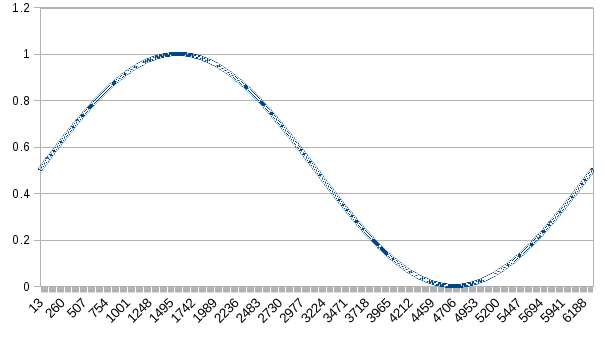
\includegraphics[width=.8\linewidth]{./images/sineApproximation/idealOutput.png}
  \caption{Ideal network output}
\end{subfigure}%
\begin{subfigure}{.5\textwidth}
  \centering
  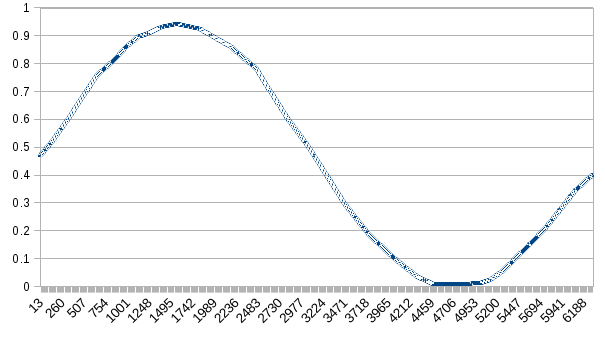
\includegraphics[width=.8\linewidth]{./images/sineApproximation/Adam50Node4LayerLeakyRELU300Batch500Iter.png}
  \caption{4 Layer Leaky RELU with 50 nodes/layer, ADAM and 500 Epocs}

\end{subfigure}
\begin{subfigure}{.5\textwidth}
  \centering
  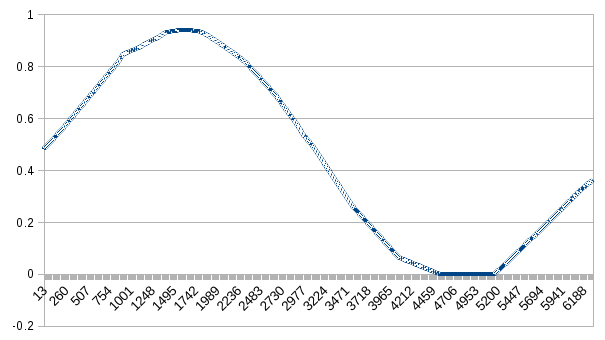
\includegraphics[width=.8\linewidth]{./images/sineApproximation/Adam25Node4LayerLeakyRELU300Batch500Iter.png}
  \caption{4 Layer Leaky RELU with 25 nodes/layer, ADAM and 500 Epocs}
\end{subfigure}
\begin{subfigure}{.5\textwidth}
  \centering
  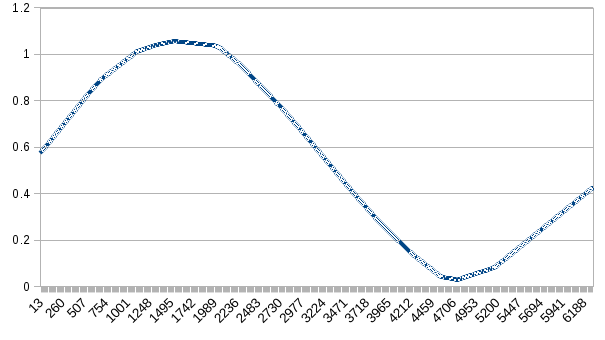
\includegraphics[width=.8\linewidth]{./images/sineApproximation/Adam25Node3LayerLeakyRELU300Batch500Iter.png}
  \caption{3 Layer Leaky RELU with 25 nodes/layer, ADAM and 500 Epocs}
\end{subfigure}

\begin{subfigure}{.5\textwidth}
  \centering
  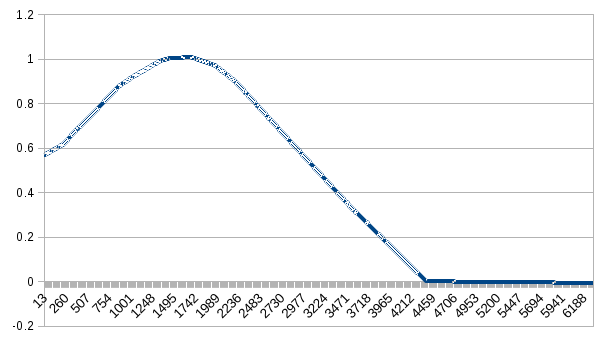
\includegraphics[width=.8\linewidth]{./images/sineApproximation/GradientDescent25Node4LayerLeakyRELU300Batch500Iter.png}
  \caption{4 Layer Leaky RELU with 50 nodes/layer, Gradient Descent and 500 Epocs}
\end{subfigure}
\begin{subfigure}{.5\textwidth}
  \centering
  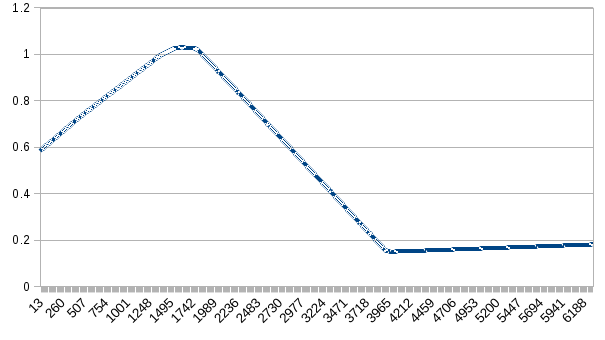
\includegraphics[width=.8\linewidth]{./images/sineApproximation/GradientDescent25Node3LayerLeakyRELU300Batch500Iter.png}
  \caption{3 Layer Leaky RELU with 25 nodes/layer, Gradient Descent and 500 Epocs}
\end{subfigure}

\caption{Approximations of the Sine Function}
\end{figure}

\subsubsection{Second Neural Network Classifier}

	Given the results of the sine approximation experiments, another attempt to make a pixel patch classifier was made.  Since the leaky RELU units had seemed more robust to settings, a 5 layer network was constructed with 75 nodes per layer (leaky RELU,  leaky RELU,  leaky RELU,  leaky RELU, linear) using the ADAM solver and mean squared error loss function.  A complication arose for the training procedure in that it was not possible to break all images into pixel patches and present them to the ADAM solver simultaneously due to RAM limitations.  This constraint meant that each training image had to be independently broken up and presented to the solver one at a time (resetting the ADAM parameters for each image).  This may have reduced training efficiency, but training the network for a day and a half resulted in a 33\% pixel error and recognizable segmentations (each image taking about 10 minutes to process).  Training for longer periods of time did not seem to remarkably improve classifier accuracy and the failure of other efforts meant that this classifier was our highest performing neural network classifier.

\subsubsection{Implementing Neural Networks with Caffe}

	We attempted to obtain access to a GPU machine and to implment a CNN using the Caffe library. We hoped for faster training/testing by using GPU augmentation. Given the difficulties creating a functional classifier with the simpler TinyCNN library, it was determined that it would be best to get the sine approximation working with the Caffe library first.\\
\\
	Many of the most prominent image data sets and challenges are focused on image classification. Potentially due to the popularity of this category of problem, the architecture of Caffe focuses on solving image classification problems.  It offer several ways of getting training data into the library, but all make the assumption that the training data is going to consist of an image and an integer label.  Many people have gotten around that restriction by directly modifying the library, but these changes do not appear to be merged to the main part of the library and documentation is severely lacking.  Despite being implemented in C++, the library seems to have a primary focus on training networks defined by JSON-like .prototxt files using images that have been processed into image databases.  This approach allows models to be easily shared between research groups and research to be conducted with a minimum of programming. However, it presents an additional obstacle to someone trying to use the library for image segmentation. Importing a network defined by a .prototxt file can trigger an assert despite the format being valid after modifications in C++.  The Caffe forum is also incredibly unresponsive, with 3 different detailed, polite and grammatically correct questions from the authors going completely unanswered.  In addition, it is somewhat difficult to take a Caffe neural net and separate it from its training apparatus (training data source, loss function, solver).

\subsubsection{Sine Approximation with Caffe}
	The sine approximation turned out to be remarkably difficult to get working as it is different from the main use case for Caffe.  Investigation into the source code for the library was required before it became possible to load the sine function training data into a RAM based Memory Data Layer.  Further investigation revealed that it is necessary to define two versions of the network to be trained and then share the weights from the training network to the test network implementation by passing the Protobuf object that defines it (otherwise it is not possible to get output from the network).  With further work it was possible to replicate the settings that had been successful with TinyCNN.  Despite only using a single processor, Caffe appears to be significantly faster than TinyCNN.

\subsubsection{Designing a Convolutional Neural Network Classifier}

	Image classification using CNNs have traditionally used architectures which have number of convolution and max-pooling layers followed by a fully connected layer.  There has been a progressive trend toward deeper networks with more convolutional layers.  This trend culminated in the development of ResNet, which is a 144-layer fully convolutional network which had the best accuracy on the 2015 ImageNet benchmark.  One of the unique innovations in ResNet was the creation of skip layers \cite{he2015deep}. These layersforwarded the results of earlier layers to later layers, allowing gradients to flow from the output layer to extremely deep layers.\\ 
\\
	The success of ResNet inspired the creation of a simple convolutional network that could hopefully deliver high performance by being able to take into account patterns from a large portion of the scene.  This network incorporated skip layers in a manner similar to ResNet.  However, development of this network was complicated by the singular focus of the Caffe library on image classification.  The library produced an error if the label portion of a Memory Data Layer was connected to a multidimensional output from a network, despite it being possible to create Memory Data Layers in that format in C++.  This problem was potentially resolved by creating two Memory Data Layers and piping their “source” data which was expected to be an image to both ends of the network independently.  However, this has the potential to stop the network from training if the examples from the two different data layers become out of sync.

\subsubsection{GPU Acceleration}

	Given the higher complexity of the Caffe network, we attempted to get access to GPU accelerated computers so that the training could be carried out at higher speed.  None of our personal computers had Nvidia GPUs, so the possible sources of GPU acceleration were the NC State University Electrical Engineering's Hydra cluster and the IBM Virtual computing lab.

\subsubsection{ECE's Hydra Cluster}

	Electrical Engineering's Hydra cluster makes several extremely expensive and high performance GPU computers available for students to use (including one with a $>$ \$3000 Tesla K40c).  Attempting to setup the Caffe library on one of the Hydra nodes was complicated by several factors.  Unlike cloud services such as Amazon's EC2, users of Hydra nodes are not granted root access to the machine.  This means it is not possible to install libraries on the system using the package manager.  This is not an insurmountable challenge as the (many) dependencies of Caffe can be downloaded and compiled manually.  However, the manual download and install process is complicated by the fact that the libraries cannot be installed to the machine and ECE students are only granted 2 Gigabytes of disk space on the network.  This requires the libraries to be downloaded to the machine's temp folder, compiled and then installed in the user's folder (updating all of the shell's environmental variables to point to the new folders where the libraries were installed).  This configuration process took more than a day and required some manual changes to the cmake files of the Caffe project. However it allowed the Caffe library to be installed locally.\\
\\
	In parallel to the manual compilation/install method, a request was also sent to the administrator of the cluster asking that the packages required by Caffe be installed via the package manager.  Around the same time as the manual compilation was finished, these packages where installed on one machine.  However, the operating system of the Hydra nodes is out of date (at least two releases behind the current) and the packages that were installed turned out to be too old to be used with the Caffe library, while the files which determined which libraries Caffe tried to used are only alterable by root.  This effectively locked out Caffe from compilation on the node where the packages where installed.  Requests to the administrator to update the Hydra node went unanswered, so Caffe was manually installed on a different node in the cluster.  However, it was discovered that the compiler on the Hydra node was also out of date and could not compile the C++11 code that had been written for the project.  These combined problems lead the Hydra cluster to be deemed not to be usable within the timeframe of the project.

\subsubsection{IBM Virtual Computing Lab}
	Another option available to us was the IBM Virtual Computing Lab. It was called a cloud service and claims had been made that it had GPU compute nodes.  Investigation revealed that it was more similar to NC State's Virtual Computing Lab then Amazon's EC2 service and that it did not have GPU compute nodes available.  It also did not have modern Ubuntu images available, leading to dated library problem similar to the Hydra cluster.  Attempts to update an Ubuntu distribution image to a more recent version simply lead to the image becoming inaccessible (it is generally not advised to do an operating system upgrades via SSH).  In any case, it is not possible for a student user to save a machine image so even if the operating system update had been successful it would have to be done again as soon as the 2 day max reservation expired.  In the end, it was decided that it would be more fruitful simply to run the software on a non-GPU laptop.

	\subsubsection{Training Convolutional Neural Networks with a CPU}

	The ResNet-inspired CNN was trained for a day and a half on a Thinkpad laptop.  Its segmentations appeared to be random noise, so the network was simplified, reducing both the number of layers and  number of filters in each layer.  This new network was also trained for one and a half days.  However, it also just produced random noise as its segmentation.  As the duration of the project was nearing an end and it seemed probable that an issue with Caffe was causing the problem, it was decided to focus on the TinyCNN based fully connected neural network.  It was trained for an additional 3 days, ultimately delivering a per pixel classification error of 33.9%.
	\subsection{SVM}
	\subsubsection{Parameter Choice} In the case of using SVM on linearly non-separable data, we played with a parameter, C, which related to the extent of wrongly categorized data points (this parameter when set to 0 assumes linearly separable data).\\
\\
	The parameters we tuned when using radial basis functions were C and $\gamma$. 
The lower the C parameter, the smoother the decision line surface. A high value for C tries to classify all training examples
correctly by allowing more training samples to be selected as support vectors. This makes the decision line much less smooth. It should
be noted that a higher C value is correlated with a higher computational time. 
The other parameter associated with the RBF kernel is gamma. The classification was very sensitive to gamma. Setting gamma to a value too small, does 
not capture the shape of the data, making it more difficult to become linearly seperable when the data is projected to a lower dimension. 
Smaller values of gamma allow for linear seperability. If a model is too smooth, which may correspond to low values of gamma, and possibly increase in 
mis-predictions C may be increased to improve the data's complexity and shape. 
For this project C and gamma were varied on a logarithmic scale from $10^{-5}$ to $10^5$ as a way to decide on the optimal parameters for accurate classification.

	\subsubsection{Implementation}
<<<<<<< HEAD
	We implemented the SVM using OpenCV's SVM functions. We ran the SVM using a linear classifier with parameters set for a linearly non-separable dataset. We also tested SVM using radial basis functions which assume non-linearly separable classes.\\
	\\ 
	OpenCV is an open sourced library of functions available in C, C++, python and java. The library we used to implement the SVM was the machine learning library using C++. Overall opencv is a great tool, with wonderful documentation although the
	learning curve on using such tools is steep for someone using them for the first time.\\
	\\
	Three features were extracted from each pixel of an the training images. The features were blue, green and red values between 0 and 255. The feature vectors were
	converted into floating point numbers in order to be used to train the SVM. The order of
	the images were shuffled randomly each time the SVM was run in order to have valid results. 
=======
	OpenCV is an open sourced library of functions available in C, C++, python and java. The library we used to implement the SVM was the machine learning library using C++. Overall opencv is a great tool, with wonderful documentation although the 
learning curve on using such tools is steep for someone using them for the first time. OpenCV requires a set of training samples which were provided as a set of images that accompanied the orignal water and not water photos. For every image in the training set, there was a bitmask image equivalent which darkened the water. These helped us provide labels for each pixel
in the training data which was given to the SVM. 
	We implemented the SVM using OpenCV's SVM functions. We ran the SVM using a linear classifier with parameters set for a linearly non-separable dataset. We also tested SVM using radial basis functions which assume non-linearly separable classes. 
	Three features were extracted from each pixel of an the training images. The features were blue, green and red values between 0 and 255. The feature vectors were 
converted into floating point numbers in order to be used to train the SVM. Due to the large number of pixels these images had in their current resolution, the training process hours.  The order of 
the images were shuffled randomly each time the SVM was run in order to have valid results. 
>>>>>>> 6d607c3bd9f111e20b0096b1f0dc5451ad9fff57
	\subsection{Detecting and Classifying "Water" vs. "Non-water" Regions}
	\subsubsection{Features Chosen}
	All work on features was performed in MATLAB, in some cases in the IBM Virtual Computing Lab. We had only the Image Processing toolbox available. For this reason, we focused on color spaces and gradient. In Project 1 we focused exclusively on the RGB ("Red/Green/Blue") color space. We decided to see if other color spaces could provide additional useful information. We also decided to include the magitude and direction of the gradient. Since areas of water generally don't have a lot of edges, we hoped that this would help identify water. Color spaces used were RGB, HSV (Hue/Saturation/Value) and YCbCr which provides luminance (Y) and chrominance (Cb and Cr) information.\\
	\subsubsection{Scatter Matrices}
	Scatter matrices provide information on the cohesion and separation of data points in different classes. The within class scatter matrix, $S_w$, provides information about how close the data points are to their center. The between class scatter matrix, $S_b$, provides information on how close the centers of each class are to each other. The mixture scatter matrix is just $S_w + S_b$.\\
\\
	An ideal situation would be one where $S_w$ has very small values and $S_b$ has very large values. This would indicate that the datapoints for the classes were very cohesive and that the classes were well separated. 
	A general measure that can be gained using the scatter matrices is called $J3=trace{S_w^{-1}S_m}$. Large values of this measure correlate with data which is well clustered and separated.
	\subsubsection{Principal Components Analysis}
	Principal Components Analysis (PCA) (also known as the Karhunen-Loeve Transform)is a way to transform data such that it is expressed in terms of the dimensions of greatest variance\cite{Shlens2003pca}. PCA can be used to reduce the redundancy and noise in a dataset. PCA can be performed in a couple of ways: one uses the eigenvectors of the covariance matrix of the variables and the other uses Singular Value Decomposition to identify a basis for the transformation. Ultimately the goal of PCA is to generate mutually uncorrelated sets of variables\cite{theodoridis2009pattern}.
	\subsection{Unsupervised Clustering}
	In Project 1 we utilized k-means to cluster data points which were labeled as water pixels. We were hoping that by creating two clusters of water pixels, we might be able to identify river bed. However, it seemed as if k-means identified shadows on the water more consistently.  In this project, we are asked to propose an unsupervised technique. We propose clustering all pixels in an image regardless of their label into one of two clusterings. We used k-means. We also clustered several images into three clusters to see if we could discern water vs. land vs. sky. The only parameter we need to set for k-means is the number of clusters. We also chose to use the dissimilarity measure of Euclidean distance for this algorithm.
	
	
\section{Results}
	\subsection{Neural Networks}
	Ultimately, the neural network solution did not offer as high accuracy as the per pixel Bayesian classifier, despite looking at 5x5 patches rather than just single pixels.  There are several possible causes for this.  The most probably is that the network used was just too small.  The initial layer was only 75 nodes, which translates to only really being able to look at 75 features of the data.  In contrast, the per pixel classifier was able to look at the 255*255*255 different possible colors of the pixel and make decisions based on its specific shade.  Even if the network was able to just focus on the middle pixel, it would not be able to notice as fine grain details as the Bayesian classifier.  While the obvious solution would be to increase the size of the network, there is a quadratic slowdown in the training speed as the number of nodes per layer is increased.  Given the amount of time that it takes the network to process a single image, that makes significantly increasing the network size difficult.  GPU acceleration would get around this issue, but does not seem to be an option at this time.
\newpage
\begin{figure}[h]
\begin{subfigure}{.33\textwidth}
  \centering
  \includegraphics[width=.9\linewidth]{./images/sourceImages/9731928435_8f83f7253e.png}
  \caption{Original Image}
\end{subfigure}%
\begin{subfigure}{.33\textwidth}
  \centering
  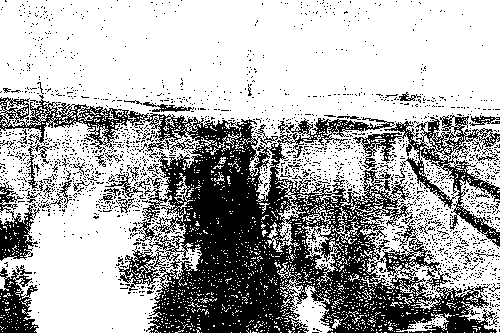
\includegraphics[width=.9\linewidth]{./images/perPixelBayesianClassifierPrimaryResults/9731928435_8f83f7253e.png}
  \caption{Per Pixel Bayesian Result}
\end{subfigure}%
\begin{subfigure}{.33\textwidth}
  \centering
  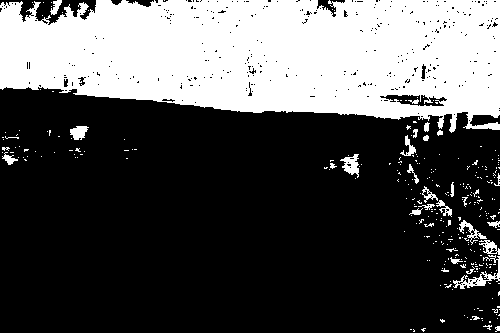
\includegraphics[width=.9\linewidth]{./images/NeuralNetworkClassifierpt339602PrimaryResults25NodeLayers/9731928435_8f83f7253e.png}
  \caption{Neural Network Result}
\end{subfigure}%

\begin{subfigure}{.33\textwidth}
  \centering
  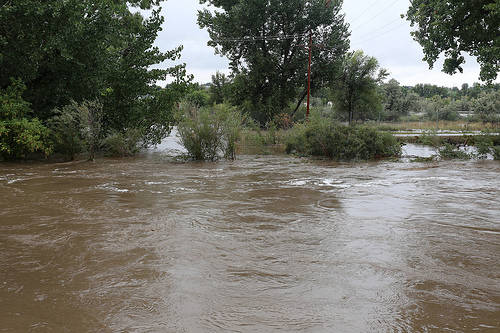
\includegraphics[width=.9\linewidth]{./images/sourceImages/9735153100_74810bbe65.png}
  \caption{Original Image}
\end{subfigure}%
\begin{subfigure}{.33\textwidth}
  \centering
  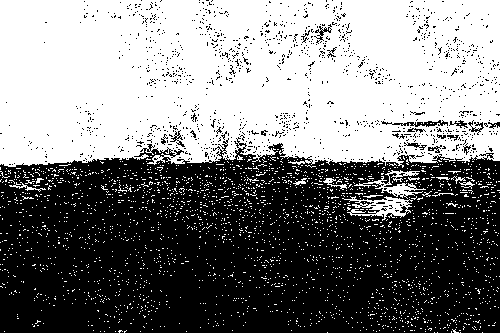
\includegraphics[width=.9\linewidth]{./images/perPixelBayesianClassifierPrimaryResults/9735153100_74810bbe65.png}
  \caption{Per Pixel Bayesian Result}
\end{subfigure}%
\begin{subfigure}{.33\textwidth}
  \centering
  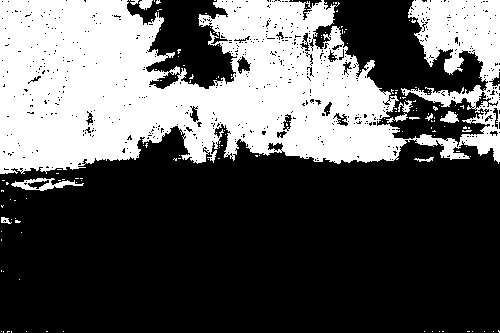
\includegraphics[width=.9\linewidth]{./images/NeuralNetworkClassifierpt339602PrimaryResults25NodeLayers/9735153100_74810bbe65.png}
  \caption{Neural Network Result}
\end{subfigure}%

\begin{subfigure}{.33\textwidth}
  \centering
  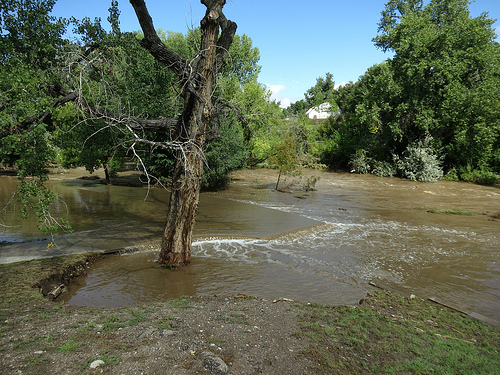
\includegraphics[width=.9\linewidth]{./images/sourceImages/9780984764_7863c32b65.png}
  \caption{Original Image}
\end{subfigure}%
\begin{subfigure}{.33\textwidth}
  \centering
  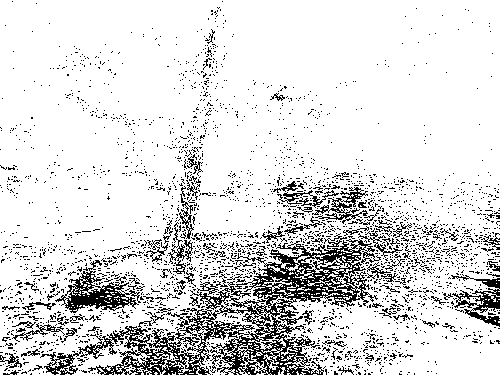
\includegraphics[width=.9\linewidth]{./images/perPixelBayesianClassifierPrimaryResults/9780984764_7863c32b65.png}
  \caption{Per Pixel Bayesian Result}
\end{subfigure}%
\begin{subfigure}{.33\textwidth}
  \centering
  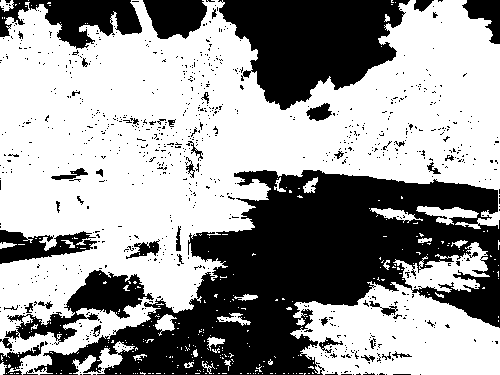
\includegraphics[width=.9\linewidth]{./images/NeuralNetworkClassifierpt339602PrimaryResults25NodeLayers/9780984764_7863c32b65.png}
  \caption{Neural Network Result}
\end{subfigure}%

\end{figure}
	While the per pixel Bayesian classifier outperformed the neural network classifier, there are some interesting differences between their output.  In general, the neural network classifier was much more consistent in its choices due to looking at multiple pixels in the image.  It also tended to deal better with reflections.  That said, it had trouble telling the difference between water and sky and still only examined a small portion of the scene.  Overall, the neural network approach appears to have significant promise (particularly if it is possible to adapt the lower levels of a professional convolutional network), but technical limitations made it difficult to realize that potential in the context of this project.
	\newpage
	\subsection{SVM}

Overall SVM performed worse then convolutional nueral networks, and Baye's theorem. Surprisingly the Linear seperator, with a parameter C did better than the radial basis function. The classification results increased in accuracy up to C = 1000 with an error rate from .37 to .42 from several runs for the linear separator, then later reached diminishing returns for any values higher than that. Computationally, it should be noted that the linear classifier took half the amount of time to train and run than the radial basis function. Below are some pictures which describe the changes: 
\begin{figure}[h]
\centering
\begin{subfigure}{.33\textwidth}
	  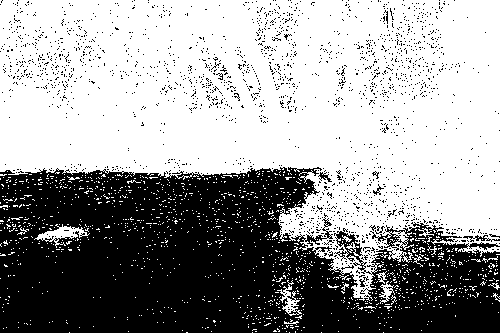
\includegraphics[width=.9\linewidth]{./images/svm/bayvSvm.png}
	  \caption{Baye's Classifier}
	\end{subfigure}%
	
\begin{subfigure}{.33\textwidth}
	  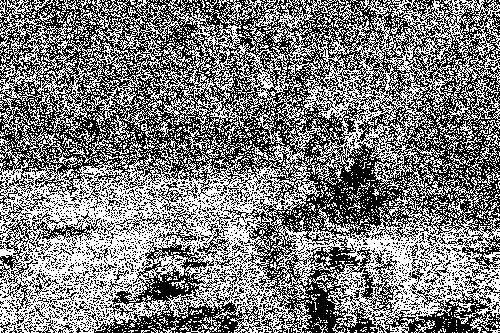
\includegraphics[width=.9\linewidth]{./images/svm/rbf.png}
	  \caption{SVM using RBF for a kernel}
	\end{subfigure}%
	
\begin{subfigure}{.33\textwidth}
	  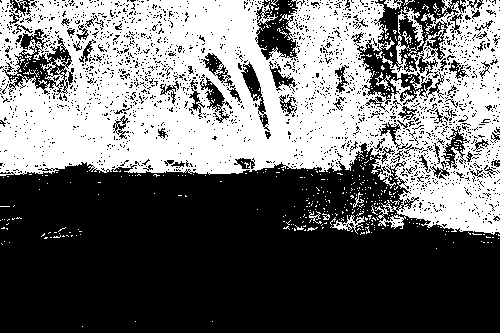
\includegraphics[width=.9\linewidth]{./images/svm/linearSvm.png}
	  \caption{Non linear SVM}
	\end{subfigure}%
	\end{figure}	
	
	\subsection{Detecting and Classifying "Water" vs. "Non-water" Regions}
	\subsubsection{Scatter Matrices}
	During Project 1 we were very aware that using RGB as a feature did not lead to highly separable classes. However, even in light of this limitation we were still able to get a per image and per pixel error rate of between .2 and .3 (sometimes even less). Due to time and resource restrictions, we limited our investigation of feature vectors in Project 2 to the gradient and color spaces.\\
	\\ 
	We calculated the scatter matrices for 11 variables: Hue, Saturation, Value, Red, Green, Blue, Y (luminence), Cr and Cb (chrominance) and two variables that describe gradient: Magnitude and Direction. \\
	\\
	We calculated the following values for the data:
	\begin{table}[h]
		\centering
		\begin{tabular}{|l|c|}
		\hline
		Measure & Value\\
		\hline
		Trace-Within-Cluster Scatter Matrix & $2.9610 \times 10^4$\\
		Trace-Between-Cluster Scatter Matrix & $34.1470$\\
		J3 & 11.2405\\
		\hline
		\end{tabular}
		\caption{Measures on 11 Data Variables}
	\end{table}
	For comparison, I refer to the results from Homework 4 in which we calculated the scatter matrices and J3 value on synthetic data in which the clusters were tightly bound situated far from each other. In this case, we got a J3 value of $9.7753 \times 10^3$. While this value comes from idealized data, it is safe to say that our J3 value suggests that we do not have cohesive and separated clusters.\\
\\
	We compared combinations of data to see how the J3 value changed depending on which variables we kept. The table below shows the results:\\
	\begin{table}[h]
		\centering
		\begin{tabular}{|c|c|c|c|}
			\hline
			All Variables & HSV & RGB & CYK\\
			\hline
			\hline
			11.2405 & 3.1427 & 3.1504 & 3.1503\\
			& & &\\
			\hline
			Gradient & RGB \& Gradient & CYK \& Gradient & HSV \& Gradient\\	
			\hline
			\hline
			2.0181 & 5.1663 & 5.1662 & 5.1559	\\
			\hline
		\end{tabular}
		\caption{J3 values for different sets of variables}
	\end{table}
	\subsubsection{PCA}
	Using MATLAB's pca() function we were able to extract the first two principal components for our data. These two components are shown in the figure below.
	\begin{figure}[h]
		\centering
		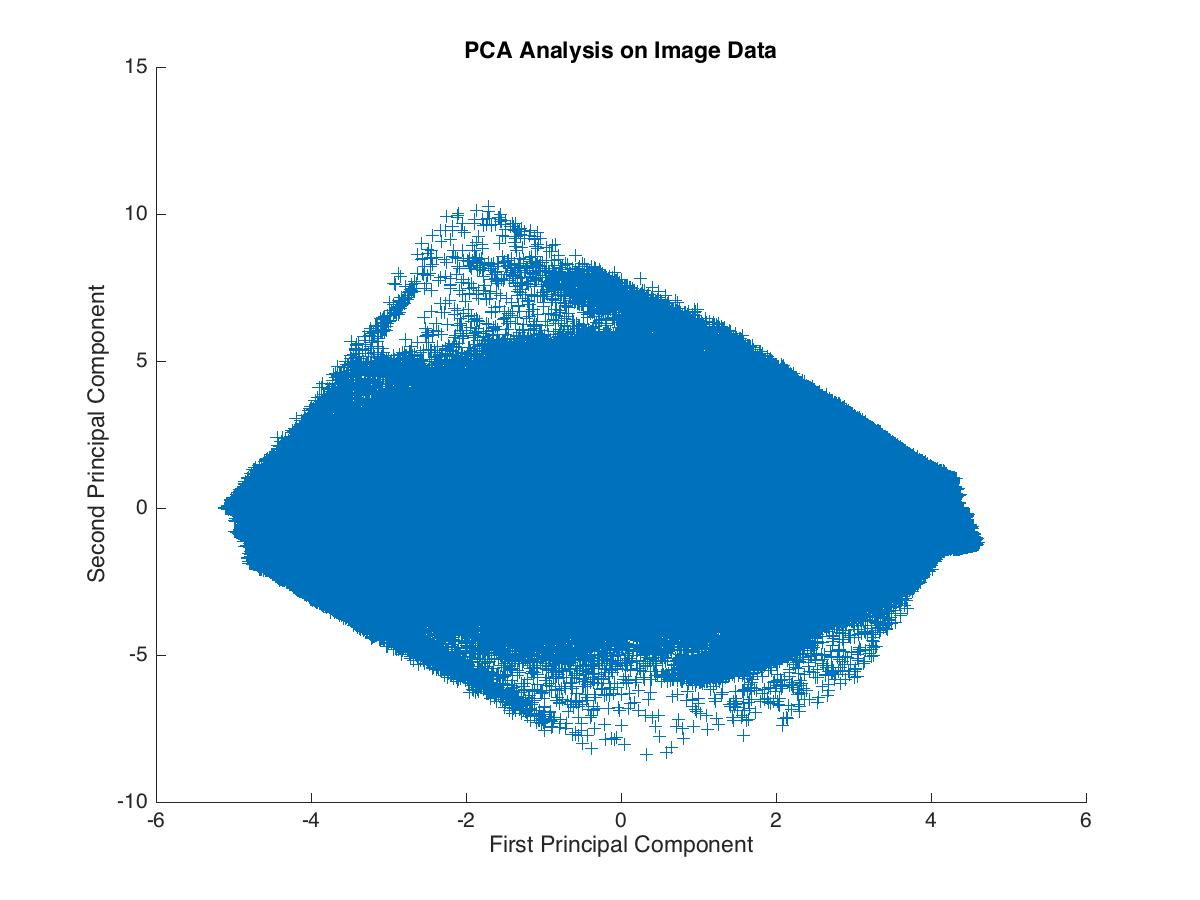
\includegraphics[scale=.25]{./images/PCA_Analysis.jpg}
		\caption{The two principal components identified using MATLAB's pca()}
	\end{figure}
	The figure shows that these two components are highly uncorrelated. MATLAB indicated that 49.9\% of the variance in the data was explained by the first principal component, while 17.8\% of the variance was explained by the second component. 
	\subsection{Unsupervised Clustering}
	We chose to run k-means with k = 2 and k = 3 so that images were segmented into 2 or 3 partitions using the dissimilarity metric Euclidean distance. While it would be ideal if 2 clusters ended up being water and not water for two clusters. In general this did not happen.  Increasing k to 3 did not segment images into water, land and sky as hoped.  In fact in some ways the 3 clusters were less meaningful than than two clusters since in the case of two clusters, water was usually delineated, but was clustered with additional objects in the image.\\
	\\
	We show the output for one image of the effect of clustering into 2 and 3 clusters.\\
	
	\begin{figure}[h]
	\begin{subfigure}{.33\textwidth}
	  \centering
	  \includegraphics[width=.9\linewidth]{./images/clustering/9731928435_8f83f7253e.png}
	  \caption{Original Image}
	\end{subfigure}%
	\begin{subfigure}{.33\textwidth}
	  \centering
	  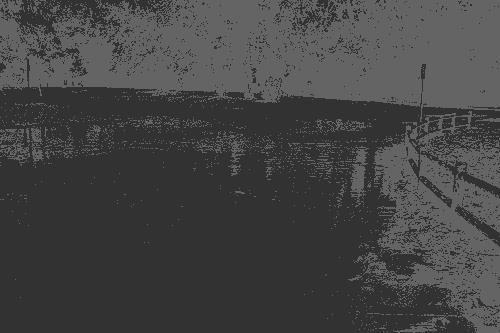
\includegraphics[width=.9\linewidth]{./images/clustering/image_23.jpg}
	  \caption{Clustered into Two Clusters}
	\end{subfigure}%
	\begin{subfigure}{.33\textwidth}
	  \centering
	  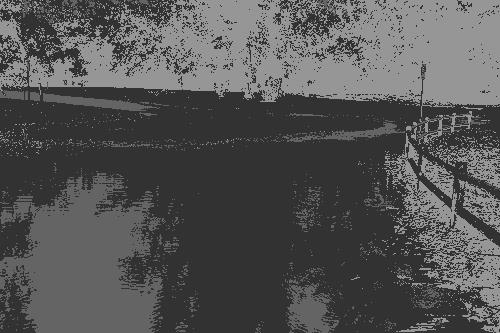
\includegraphics[width=.9\linewidth]{./images/clustering/image_32.jpg}
	  \caption{Clustered into Three Clusters}
	\end{subfigure}%
	\end{figure}
	
	It is clear that for the task of identifying water vs. non-water pixels, clustering will not automatically return in the two clusters water vs. non-water.


\section{Discussion}
In this Project we explored other classification algorithms and compared them to the Bayes Classifier.  As expected in cases where our algorithms were employing a linear separation, the Bayes Classifier performed the best. \\
\\ 
In general even though our classification problem is a highly non-linear one, the Bayes classifier did better. However, we surmise that getting more training data and/or tweaking the CNN has the potential to generate better results.\\
\\
We also discovered that clustering the data in the images using Euclidean distance was not sufficient to identify water vs. non-water pixels. Particularly increasing the number of clusters to 3 to not see a huge improvement.
For the SVM the largest limitation was how long it took to train the data. One interesting idea would be to shrink the images down, and run the SVM. 
In most classifiers including Baye's the brightness of the sky was often confused with the reflective water pixels. One idea to help with differentiating between the two would be to assign more weights to the water pixels in the training data that were less reflective. 
\newpage
\bibliographystyle{plain}
% --------------------------------------------------------------
%     You don't have to mess with anything below this line.
% --------------------------------------------------------------
 \bibliography{Refs}  
\end{document}
